\documentclass{article}
\usepackage{graphicx}
\usepackage{hyperref}
\usepackage{tabularx}
\usepackage{multirow}
\usepackage{algorithm}
\usepackage{algorithmic}
\usepackage{spverbatim}
\usepackage[colorlinks=false,linkcolor=black,urlcolor=black,bookmarksopen=true]{hyperref}
\usepackage{bookmark}
\usepackage{times}
\usepackage{comment}
\usepackage{graphicx}
\usepackage{latexsym}
\usepackage{amsmath}
\usepackage{amssymb}
\usepackage{ntheorem}
\bibliographystyle{alpha}
\begin{document}

\begin{titlepage}
	\vspace*{2cm}
  \begin{center}
   {\Large Is Science Effective at Creating Knowledge that Matters?\\
	\small Evidence from the Life Sciences\\}
   \vspace{2cm} 
   {Exposé\\}
   \vspace{2cm}
   {presented by\\
    Nahor George Gebretensae\\
		Matriculation Number 1586529\\
   }
   \vspace{1cm} 
   {submitted to the\\
    Chair of Organization and Innovation\\
		Assistant Professorship of Technological\\
		Innovation and Management Science\\
    Prof.\ Dr.\ Marc Lerchenmüller\\
    University of Mannheim\\} \vspace{2cm}
   {2020}
  \end{center}
\end{titlepage}

\newpage
\tableofcontents
\newpage
\listoftables
\newpage

\section{Problem Statement}
The funding of scientific research is almost always justified in terms of possible beneficial outcomes for the society. Most research efforts, whether public or private funded, are intended to achieve objectives which transcend science \cite{Sarewitz2007TheNH}. \\
\\
For example much of the research efforts supported by the U.S. National Institutes of Health (NIH) is considered to be basic since it explores the fundamental phenomena of human biology. The public support of the NIH is tied to the expectation and legislative mandate that the research result should end up improving human health \cite{Sarewitz2007TheNH}. \\
\\
In \textit{The applied value of public investments in biomedical research}\cite{Li2017TheAV} Li et al. discovered links between public research investments conducted by NIH and subsequent patenting: 10\% of NIH grants directly generated patents and 30\% of NIH grants were cited in patents. Because of the lack of a yardstick it is unclear whether 30\% are a lot or not \cite{Li2017TheAV}. The question, if a certain research effort is effective, seems to lie at the heart of science policy, but is rarely asked and much less studied systematically \cite{Sarewitz2007TheNH}. \\
\\
\textbf{Genotype and diseases.} The genotype can yield information about disease susceptibility and the effectiveness of the medication \cite{Brunicardi2011OverviewOT}. According to Spear et al.`s \textit{Clinical application of pharmacogenetics} \cite{Spear2001ClinicalAO}, it is estimated that up to 75\% of patients fail to respond to many commonly used drugs \cite{Spear2001ClinicalAO}. The effectiveness of the medication depends on the genomic characteristics of the patient: The rate at which the medication gets metabolized or the causal factors of the disease \cite{Brunicardi2011OverviewOT}. \\
\\
\textbf{Evolutionary Biology.} In \textit{Gene expression across mammalian organ development} \cite{CardosoMoreira2019GeneEA}, Cardoso-Moreira et al. profiled the development of seven organs (cerebrum, cerebellum, heart, kidney, liver, ovary and testis) from organogenesis till adulthood across multiple mammals (rhesus macaque, mouse, rat, rabbit, opossum and chicken) including humans \cite{CardosoMoreira2019GeneEA}. Comparisons of gene expression patterns in organ development within and across mammals identified correspondences of developmental stages across species. Moreover recent evolutionary biology data reveal, however, that genes that influence diseases may express differently in animals versus humans \cite{CardosoMoreira2019GeneEA}. This thesis will only focus on comparison of gene behavior between humans and mice.\\
\\
\textbf{Yardstick for assessing efficacy of knowledge creation.} This recent data allows an assessment of whether the scientific research enterprise primarily targets genes that work similarly in humans versus animals and hence seem more promising. This essentially offers a yardstick against which to assess the efficacy of knowledge creation in the life sciences.

\section{Datasets}
\subsection{Kaessmann Group Datasets}
\label{kaessmann}
Kaessmann Group Datasets are provided by the \href{https://www.zmbh.uni-heidelberg.de/kaessmann/}{Kaessmann Group} and contain data on comparison of gene behavior between humans and mice. \cite{CardosoMoreira2019GeneEA}.

\begin{table}[!ht]
\centering
\setlength\extrarowheight{2pt} % for a bit of visual "breathing space"
\begin{footnotesize}
\begin{tabularx}{\textwidth}{|l|l|l|l|l|l|}
\hline
\textbf{File} & \textbf{Source} & \textbf{Format} & \textbf{Class} & \textbf{Entities} & \textbf{Attributes} & \\ \hline
\href{https://nahorgebre.s3.amazonaws.com/Brain.csv}{Brain} & \href{https://www.zmbh.uni-heidelberg.de/kaessmann/}{Kaessmann Group}  & csv & Gene & 8.334 & 4 \\
\href{https://nahorgebre.s3.amazonaws.com/mart_export_brain.txt}{mart\_export\_brain} & \href{https://www.zmbh.uni-heidelberg.de/kaessmann/}{Kaessmann Group} & txt & Gene & 8.333 & 3 \\
\href{https://nahorgebre.s3.amazonaws.com/Cerebellum.csv}{Cerebellum} & \href{https://www.zmbh.uni-heidelberg.de/kaessmann/}{Kaessmann Group}  & csv & Gene & 7.133 & 4 \\
\href{https://nahorgebre.s3.amazonaws.com/mart_export_cerebellum.txt}{mart\_export\_cerebellum} & \href{https://www.zmbh.uni-heidelberg.de/kaessmann/}{Kaessmann Group} & txt & Gene & 7.133 & 3 \\
\href{https://nahorgebre.s3.amazonaws.com/Heart.csv}{Heart} & \href{https://www.zmbh.uni-heidelberg.de/kaessmann/}{Kaessmann Group}  & csv & Gene & 5.254 & 3 \\
\href{https://nahorgebre.s3.amazonaws.com/Heart_Ensembl_NCBI_Crosswalk.txt}{Heart\_Ensembl\_NCBI\_Crosswalk} & \href{https://www.zmbh.uni-heidelberg.de/kaessmann/}{Kaessmann Group} & txt & Gene & 5.261 & 3 \\
\href{https://nahorgebre.s3.amazonaws.com/mart_export_heart.txt}{mart\_export\_heart} & \href{https://www.zmbh.uni-heidelberg.de/kaessmann/}{Kaessmann Group} & txt & Gene & 5.254 & 3 \\
\href{https://nahorgebre.s3.amazonaws.com/Kidney.csv}{Kidney} & \href{https://www.zmbh.uni-heidelberg.de/kaessmann/}{Kaessmann Group}  & csv & Gene & 6.610 & 3 \\
\href{https://nahorgebre.s3.amazonaws.com/mart_export_kidney.txt}{mart\_export\_kidney} & \href{https://www.zmbh.uni-heidelberg.de/kaessmann/}{Kaessmann Group} & txt & Gene & 6.610 & 3 \\
\href{https://nahorgebre.s3.amazonaws.com/Liver.csv}{Liver} & \href{https://www.zmbh.uni-heidelberg.de/kaessmann/}{Kaessmann Group}  & csv & Gene & 5.742 & 4 \\
\href{https://nahorgebre.s3.amazonaws.com/mart_export_liver.txt}{mart\_export\_liver} & \href{https://www.zmbh.uni-heidelberg.de/kaessmann/}{Kaessmann Group} & txt & Gene & 5.741 & 3 \\
\href{https://nahorgebre.s3.amazonaws.com/mart_export_testis.txt}{mart\_export\_testis} & \href{https://www.zmbh.uni-heidelberg.de/kaessmann/}{Kaessmann Group} & txt & Gene & 8.666 & 3 \\
\href{https://nahorgebre.s3.amazonaws.com/Testis.csv}{Testis} & \href{https://www.zmbh.uni-heidelberg.de/kaessmann/}{Kaessmann Group}  & csv & Gene & 8.667 & 4 \\
\hline
\end{tabularx}
\end{footnotesize}
\caption{Kaessmann Group Datasets \cite{CardosoMoreira2019GeneEA}}
\end{table}

\subsection{DisGeNet Dataset}
\label{disgenet}
DisGeNet Dataset is provided by \href{https://www.disgenet.org/}{DisGeNet} and contains data on gene-disease associations. DisGeNet is a discovery platform containing one of the largest publicly available collections of genes and variants associated with human diseases \cite{Piero2019TheDK}.
 
\begin{table}[!ht]
\setlength\extrarowheight{2pt} % for a bit of visual "breathing space"
\begin{footnotesize}
\begin{tabularx}{\textwidth}{|C|C|C|C|C|C|}
\hline
\textbf{File} & \textbf{Source} & \textbf{Format} & \textbf{Class} & \textbf{Entities} & \textbf{Attributes} \\
\hline
\href{https://nahorgebre.s3.amazonaws.com/all_gene_disease_pmid_associations.tsv}{all\_gene\_disease\_pmid\_associations} & \href{https://www.disgenet.org/}{DisGeNet}  & tsv & Gene and Disease & 1.548.062 & 15 \\
\hline
\end{tabularx}
\end{footnotesize}
\caption{DisGeNet Dataset \cite{Piero2019TheDK}}
\end{table}

\subsection{USPTO Bulk Data}
\label{uspto}
The \href{https://bulkdata.uspto.gov/}{Bulk Data Storage System (BDSS)} provides a single repository for raw public bulk data on patents of the \href{https://www.uspto.gov/}{United States Patent and Trademark Office (USPTO)}. Bulk data refers to putting all static data into a file or set of files so that all of the data can be acquired with downloads \cite{Uspto}.

\subsection{PubTator Dataset}
\label{pubtator}
PubTator Central is a text mining tool for retrieving bioconcept annotations like genes from abstracts and titles of 29 million PubMed-Publications. Annotations are downloadable in multiple formats including bulk FTP \cite{Wei2019PubTatorCA}.

\subsection{RePORTER Publication Datasets}
\label{publication}
RePORTER Publication Datasets contain links between publications in PubMed and research projects of the NIH \cite{publicNIH}.

\subsection{RePORTER Patent Dataset}
\label{patent}
RePORTER Patent Dataset contains links between patents and research projects of the NIH \cite{patentNIH}.

\subsection{GPRO Gold-Standard patent corpora}
\label{gpro}
The GPRO (gene and protein-related object) gold standard corpora consist of training and development sets noted as GPRO\_T and GPRO\_D. Each of the datasets contains the title and the abstract of 7000 manually annotated patents. The manually labelled annotations are done by domain experts \cite{Krallinger2015TheCC}.

\begin{table}[!ht]
\setlength\extrarowheight{2pt} % for a bit of visual "breathing space"
\begin{footnotesize}
\begin{tabularx}{\textwidth}{|C|C|C|}
\hline
\textbf{Corpus} & \textbf{Number of Patents} & \textbf{Number of Annotations} \\
\hline
GPRO training set (GPRO\_T) ≈ 662234 token \cite{Krallinger2015TheCC} & 7000 patents (title and abstracts) & 4396 annotations \\
GPRO development set (GPRO\_D) ≈ 648732 token \cite{Krallinger2015TheCC} & 7000 patents (title and abstracts) & 3934 annotations \\
\hline
\end{tabularx}
\end{footnotesize}
\caption{Details of the gold standard patent corpora containing the annotations for genes \cite{Habibi2016PerformanceOG}}
\end{table}

\section{Contribution}

To assess the efficacy of knowledge creation, the thesis will focus on the following three contiguous research aims:
\begin{itemize}
	\item \textbf{First aim:} Does the rate of scientific knowledge creation differ for genes that function similar versus different in animals versus humans?
	\item \textbf{Second aim:} Does the rate of scientific knowledge creation differ for genes that are strongly versus weakly associated with human diseases?
	\item \textbf{Third aim:} Does patenting activity differ across the obtained gene typology?
\end{itemize}
\\
\\
To address these AIMs, I will integrate data on gene annotations from 29 million life science publications contained in the \nameref{pubtator}, on gene-disease associations contained in the \nameref{disgenet}, on patents form \nameref{uspto}, and on gene behavior information contained in the \nameref{kaessmann}. \\
\\
As one can see in figure \ref{fig:gene-topology-gene-activity}, the efficacy of knowledge creation will be assessed by counting the amount of patents across the two dimensional gene topology.

\begin{figure}
	\begin{center}
	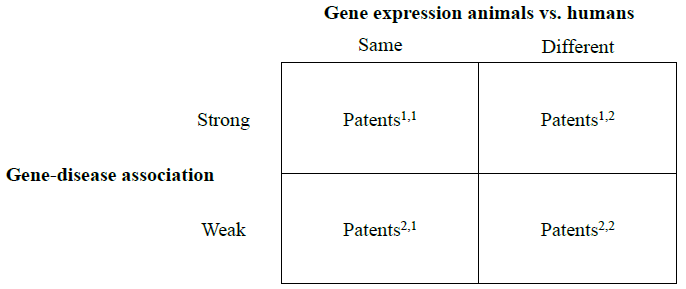
\includegraphics[width=13cm]{./gene-topology-gene-activity.png}
	\caption[Patenting activity by gene typology]{Patenting activity by gene typology}
	\label{fig:gene-topology-gene-activity}
	\end{center}
\end{figure}

\section{Workplan}
\subsection{Gene Name Recognition on Patents}
Since the process of data integration requires structured data, I will extract structured knowledge from unstructured patent text data using named entity recognition. \\
\\
\textbf{Extracting and Parsing Patent Data.} The patent data made available by the United States Patent and Trademark Office (USPTO) is formatted as XML and ASP. The aim is to apply gene name recognition approaches on \textit{title}, \textit{abstract}, \textit{description} and \textit{claims} of \href{http://patft.uspto.gov/netahtml/PTO/index.html}{300.000 patents}, filed by U.S. pharmaceutical and biotechnology firms. Therefore, I created a parser that extracts the required data from the source files. \\
\\
\textbf{Gold-Standard patent corpora.} The \nameref{gpro} contains records for patent title and abstract. Since there are no gold-standard corpora for patent description and claims available, I will generate a gold-standard dataset by integrating the following datasets: \nameref{pubtator}, \nameref{uspto}, \nameref{publication}, \nameref{patent}. \\
\\
The NIH funds roughly 80\% of all biomedical research laboratories in the United States. The thus funded research efforts lead to many patents, and researchers are required by federal law to link their research activity to ensuing patent filings \cite{Li2017TheAV}. As of June 2020, there are 29.207 such patents associated with the underpinning basic science publications through means of unique identifiers: \nameref{publication} \& \nameref{patent}. \\
\\
Using the \nameref{pubtator} dataset, I can determine which genes are occurring in these publications. The genes which are occurring in the associated publications and in the patent text are added to the gold-standard dataset.
\\
\\
\textbf{ScispaCy \& FLAIR.} \href{https://allenai.github.io/scispacy/}{ScispaCy} is a Python library for biomedical text processing, which heavily leverages the spaCy library. It was conceived as a means to automate the process of extracting gene entities from scientific papers and provides multiple pretrained models \cite{Neumann2019ScispaCyFA}. I will use the pretrained scispaCy model \textit{en\_ner\_bionlp13cg\_md} to detect all gene entities. \\
\\
\href{https://www.informatik.hu-berlin.de/de/forschung/gebiete/ml/Flair/flair}{FLAIR} is an NLP framework, which facilitates the training of state-of-the-art text classification models. I will utilize this framework to train a model for gene entity recognition \cite{Akbik2019FLAIRAE}. 

\textbf{Evaluation.} The performance of ScispaCy and FLAIR will be evaluated by comparing system predicted entities with gold-annotated entities in terms of Precision, Recall and F-Measure. \\

\subsection{Gene Data Integration}
To integrate all files I will use the \textit{WInte.r} framework. The framework supports end-to-end data integration and entails algorithms and building blocks for data loading, pre-processing, schema matching, identity resolution and data fusion \cite{Lehmberg2017WInterA}. The data integration process will consist of three steps: Data Translation, Identity Resolution and Data Fusion. In Data Translation, I will pursue the dissolution of structural heterogeneity by transferring data into a uniform target schema. In Identity Resolution, I will pursue the dissolution of the semantic heterogeneity, by finding records which describe the same real-world entity. In Data Fusion, I will consolidate duplicate records into one record. \\
\\
\textbf{Evaluation.} Comparing system predicted correspondences with gold-annotated correspondences in terms of Precision, Recall and F-Measure, I will evaluate the results of data integration.

\bibliography{source}
\end{document}